\documentclass[12pt,a4paper,openright,twoside]{report}

\usepackage[english]{babel}
\usepackage{indentfirst}
\usepackage{xcolor}
\usepackage{eucal}
\usepackage{amsmath}
\usepackage{amsfonts}
\usepackage{comment}
\usepackage{newlfont}
\usepackage[parfill]{parskip}
\usepackage{listings} 
\usepackage{hyperref}
\usepackage{marvosym}
\usepackage{csquotes}
\usepackage{subfig}
\usepackage{adjustbox}

\usepackage{algorithm}
\usepackage{algpseudocode}

% Biblatex - bibliograpy 
\usepackage[sorting=none]{biblatex}
\addbibresource{bibliography.bib}

% appendix 
\usepackage[toc,page]{appendix} 

% caption management
\usepackage[margin=1cm]{caption}

% some page formating
\usepackage[textwidth=400pt]{geometry}
\numberwithin{equation}{section} 
\linespread{1.3} 

% fancyhdr - Page format
\usepackage{fancyhdr}
\pagestyle{fancy}\addtolength{\headwidth}{20pt}
\renewcommand{\chaptermark}[1]{\markboth{\thechapter.\ #1}{}}
\renewcommand{\sectionmark}[1]{\markright{\thesection \ #1}{}}
\rhead[\fancyplain{}{\bfseries\leftmark}]{\fancyplain{}{\bfseries\thepage}}
\cfoot{}

% Tikz - Graph and diagrams
\usepackage{tikz}
\usetikzlibrary{arrows,positioning} 
\tikzset{
    %Define standard arrow tip
    >=stealth',
    %Define style for boxes
    punkt/.style={
           rectangle,
           rounded corners,
           draw=black, very thick,
           text width=6.5em,
           minimum height=2em,
           text centered},
    % Define arrow style
    pil/.style={
           ->,
           thick,
           shorten <=2pt,
           shorten >=2pt,}
}


% Json repr in listing
\colorlet{punct}{red!60!black}
\definecolor{background}{HTML}{EEEEEE}
\definecolor{delim}{RGB}{20,105,176}
\colorlet{numb}{magenta!60!black}

\lstdefinelanguage{json}{
    basicstyle=\tiny\ttfamily,
    numbers=left,
    numberstyle=\scriptsize,
    stepnumber=1,
    numbersep=8pt,
    showstringspaces=false,
    breaklines=true,
    frame=lines,
    backgroundcolor=\color{background},
    literate=
     *{0}{{{\color{numb}0}}}{1}
      {1}{{{\color{numb}1}}}{1}
      {2}{{{\color{numb}2}}}{1}
      {3}{{{\color{numb}3}}}{1}
      {4}{{{\color{numb}4}}}{1}
      {5}{{{\color{numb}5}}}{1}
      {6}{{{\color{numb}6}}}{1}
      {7}{{{\color{numb}7}}}{1}
      {8}{{{\color{numb}8}}}{1}
      {9}{{{\color{numb}9}}}{1}
      {:}{{{\color{punct}{:}}}}{1}
      {,}{{{\color{punct}{,}}}}{1}
      {\{}{{{\color{delim}{\{}}}}{1}
      {\}}{{{\color{delim}{\}}}}}{1}
      {[}{{{\color{delim}{[}}}}{1}
      {]}{{{\color{delim}{]}}}}{1},
}


% ragged2e - Justifying text
\usepackage{ragged2e}
\justifying


\begin{document} 



\begin{titlepage}
    \textwidth=450pt\oddsidemargin=0pt
    \begin{center}
    {{\Large{\textsc{Alma Mater Studiorum $\cdot$ Universit\`a di
    Bologna}}}} \rule[0.1cm]{15.8cm}{0.1mm}
    \rule[0.5cm]{15.8cm}{0.6mm}
    {\small{\bf SCUOLA DI SCIENZE\\
    Corso di Laurea in Nome corso di Laurea }}
    \end{center}
    \vspace{15mm}
    \begin{center}
    {\Large{\bf A STUDY ON TAXATION POLICY}}\\
    \vspace{3mm}
    {\Large{\bf   ON HETEROGENEOUS }}\\
    \vspace{3mm}
    {\Large{\bf NON-ANALITICAL BEHAVING AGENTS}}\\
    \end{center}
    \vspace{40mm}
    \par
    \noindent
    \begin{minipage}[t]{0.47\textwidth}
    {\large{\bf Relatore:\\
    Chiar.mo Prof.\\
    NOME RELATORE}}
    \end{minipage}
    \hfill
    \begin{minipage}[t]{0.47\textwidth}\raggedleft
    {\large{\bf Presentata da:\\
    NOME LAUREANDO}}
    \end{minipage}
    \vspace{20mm}
    \begin{center}
    {\large{\bf Sessione\\%inserire il numero della sessione in cui ci si laurea
    Anno Accademico }}%inserire l'anno accademico a cui si � iscritti
    \end{center}
    \end{titlepage}

\begin{comment}

%------------------------------------------------------------------------------------
% TITLE PAGE
%------------------------------------------------------------------------------------
\begin{titlepage} 
\thispagestyle{empty}                   %elimina il numero della pagina
\topmargin=6.5cm                        %imposta il margina superiore a 6.5cm
\raggedleft                             %incolonna la scrittura a destra
\large                                  %aumenta la grandezza del carattere
\em                                     %emfatizza (corsivo) il carattere
Questa è la \textsc{Dedica}:\\
ognuno può scrivere quello che vuole, \\
anche nulla \ldots                   
\newpage                               
%\clearpage{\pagestyle{empty}\cleardoublepage}%non numera l'ultima pagina sinistra
\end{titlepage}
%------------------------------------------------------------------------------------
       
\end{comment}



%------------------------------------------------------------------------------------
% INTRO - TABLE OF CONTENTS
%------------------------------------------------------------------------------------
\pagenumbering{roman}                  
\chapter*{Abstract}             
\addcontentsline{toc}{chapter}{Abstract}

The work presents a set of economical simulations through AI-driven agents that maximises their utility. This is done using a python package called Foundation and

\clearpage{\pagestyle{empty}\cleardoublepage}
\tableofcontents      
\clearpage{\pagestyle{empty}\cleardoublepage}

\begingroup
\let\clearpage\relax
\listoffigures   
\listoftables  
\endgroup

\clearpage{\pagestyle{empty}\cleardoublepage}

\pagenumbering{arabic}
%------------------------------------------------------------------------------------
\chapter*{Introduction}             
\addcontentsline{toc}{chapter}{Introduction}

One of the challenges in macroeconomic theory is to transpose the theory to the real world. In particular the process of designing a policy and implementing it. This is because the analytical solutions are bounded to certain a level of complexity. The more complex and similar to reality the problem gets the harder it gets to solve it analytically. In addition agents are heterogeneous and thus each one is acting differently according to his skill and initial state. 


In this thesis I am going to present a partial reproduction with expansion of the paper \textit{The AI Economist: Optimal Economic Policy Design via Two-level Deep Reinforcement Learning}\cite{zheng2021ai}. With the scope of presenting an AI-driven economical simulation, where is possible to investigate high complexity setup that would be almost impossible to study analytically. It will be shown that AI-driven agents are able to come up with emerging behaviors and specialization in order to maximize their own utility. Afterward multiple kind of taxation will be introduced in the simulations as a discriminant factor, and we will compare the results on total economical productivity and on coin equality among agents.



%------------------------------------------------------------------------------------
% CHAPTER 1
%------------------------------------------------------------------------------------
\chapter{What is Foundation}
In this chapter, I am going to introduce the package developed by Alex Trott and Stephen Zheng and provided by Salesforce called Foundation\cite{zheng2020ai}. This package offers the possibility to create simulations with multiple agents that interact in a 2D world. At first, there will be a presentation of the gather-and-build simulation with the relevant entities and dynamics. Furthermore, the basic agents will be dismantled in their main components to better understand their action space and scope, and finally, there will be a small discussion on the behavior of the policymaker.

\section{Gather and trade}

The simulation that will be used through the dissertation is called gather and trade. This simulation takes place in a 2D map that represents the world where the agents live and interact. The shape of the world is a 25x25 grid where are disposed various kinds of entities. Within this world, 4 agents are free to move around, gather resources, trade them and use them to build houses. These agents are different for their skill level, allowing them to have higher/lower rewards for their actions. A fifth agent, called policymaker, is asked to tax and redistribute the income of the four previous agents, based on information about their endowments, but not their skill.

\subsection{World and entities}

As aforementioned the map is a 25x25 grid where are present some entities. Some of these are visible in the world as water or stone, others are just present in the agent's endowment as coins or labour. The complete set of entities is:

\begin{itemize}
    \item Water
    \item House
    \item Source Block (Wood and Stone)
    \item Wood and Stone
    \item Coins
    \item Labor
\end{itemize}

Water is a simple world block that has no use other than avoiding agents passing through. We can see from Figure \ref{img:map_0} that the water is used to divide the world into 4 macro-areas, each one with different resources. 
A House is a block that is not present at the beginning of the simulation, but it can be built by agents in an empty block, only the owner of the house can walk through it.

Source blocks are two entities that spawn stochastically resources, namely wood, and stone, as we can see from Figure \ref{img:map_0} in the four areas divided by the water we have a zone with both wood and stone source block, two other areas with just one kind of source block and one that has no resources at all. 

Coins are the measurement of the value produced in the world. Coins are generated when a house is built, the agent that builds the house is rewarded with a certain amount of coins that varies with the skill level.

Labor is a measurement of the total effort exerted by an agent, it is generated every time an agent takes an action and is percieved as a dis-utility from the agent.


\begin{figure}[h!]
    \centering
    \linespread{.9} 
    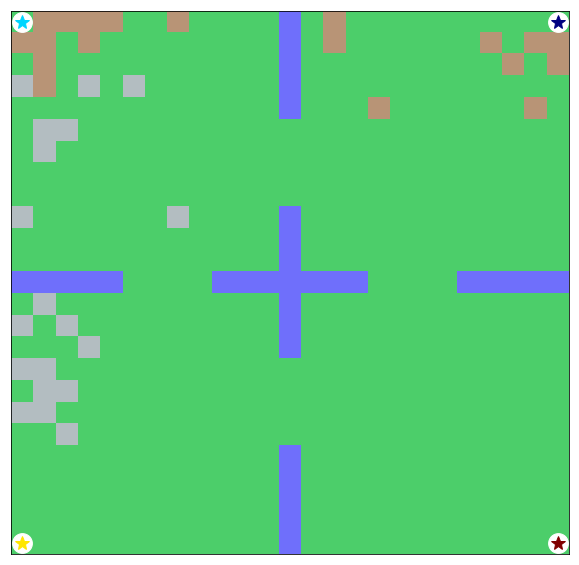
\includegraphics[width=0.5\textwidth]{Resources/imgs/Map_0.png}
    \caption[Rendering of the world at inital conditions: ]%
    {\label{img:map_0}Rendering of the world at inital conditions: \small \textit{this is a rendering of the world map at the first timestep of the simulation, blue blocks are water, brown blocks are wood sources, grey blocks are Stone sources. The four corners are the starting positions for the 4 agents.}}
\end{figure}



\subsection{Game dynamics}

A problem that has a continuous flow of agent-environment interactions can be formalized by a Finite Markov Decision problem \cite{sutton2018reinforcement}. In particular, this simulation is a partial-observable multi-agent Markov Games (MGs). The problem is defined by the tuple \(\left(  S,A,R ,\gamma, o, \mathcal{T} \right) \) where \( S \) is the state space, \( A \) is the action space, \( R \) the reward space and gamma a dicount factor. 

The simulation is composed of a series of episodes, each of length \( H \) time-steps. At every point in time \( t \in [0,H] \) the episode is characterized by a state \( s_t \), representing the current world environment, every agent performs an action \( a_{i,t}  \)  given the current partial observation \( o_{i,t}\) of the world state, and receives a reward \( r_{it}  \). Afterwards the environment transits to a new state \( s_{t+1} \) according to the transition distribution \(  \mathcal{T}(s_{t+1}|s_t,\boldsymbol{a}_t)\). This chain of interactions state-action-reward/state carries on until the end of an episode.

\begin{equation*}
     s_0 \,  \rightarrow_{\boldsymbol{o}_0}\, \boldsymbol{a}_0 \,\rightarrow\, r_1 , s_1 \,\rightarrow_{\boldsymbol{o}_1}\, \boldsymbol{a}_1 \,\rightarrow ... \rightarrow_{\boldsymbol{o}_{H-1}}\, \boldsymbol{a}_{H-1} \,\rightarrow\, r_H , s_H
\end{equation*}

Here \( \boldsymbol{a} \) and \( \boldsymbol{o} \) are the vectorized observations and actions for all the five agents. Given the particular structure of the simulation every single agent will receive an observation at every time-step (different for everyone, more on that later), but only at the 4 basic agents will be asked to act, the policymaker will act only upon a certain condition met. In this case, the episode lasts for 1000 time-step and the policymaker is asked to act (tax the other agents) every other 100 steps. The existence of multiple episodes is necessary for the 4 agents and the policymaker to define their own optimal policy \( \pi_i(o_{i,t}, h_{i,t-1};\theta_i^*) \), this optimization process will be discussed in the RL chapter.

\subsection{Agents}

Fromthe information above we know that the four basic agents are endowed with labor, coins, wood and stone. They live in the world map, can act within it and their objective is to maximize their $\gamma$-discounted utility function. Now I will describe in more detail the agents starting from the information that they receive at each time-step, then talking about the actions that they are allowed to take and finally about their objective. 

\paragraph{Observation space:} Given that this simulation is a partial-observable multi-agent Markov Game, the observation that agent \( i \) receive at time \( t \) is not complete but partial, this information can be summarized in the following way:

\begin{itemize}
    \item \(o_{i,t}^{\text{world state}}\): world map situation surrounding the agent, this is limited to the 11x11 grid around the agent \( i \).
    \item \(o_{i,t}^{\text{market state}}\): full information about the market state for wood, stone and available trades.
    \item \(o_{i,t}^{\text{agent}}\): public resources and coin endowments (this information is also available to the policy maker), private labor performed and skill level.
    \item \( o_{i,t}^{\text{tax}} \): tax structure
    \item \( o_{i,t}^{\text{other}} \): other information (ex. action mask)
\end{itemize}
 
the full observation space can be seen in Table \ref{tab:full_obs}

\paragraph{Action space:} The agent can take one action per time-step and can choose this action from the 50 listed below:

\begin{itemize}
    \item \textbf{Movement}: 4 actions for the basic movements N, S, E, W
    \item \textbf{Gather}: 1 action for gathering resources
    \item \textbf{Trade}: 44 actions for trading resources
    \item \textbf{Idle}: 1 action that does nothing
\end{itemize}

The movement's actions along with gather do not need much of an explanation, these are simple actions that increases labor by 0.21 units each time pursued. The building action requires the agent to consume (destroy) one unit of wood and one unit of Stone, as a consequence he gains 2.1 units of labor and an amount of coin that depends on his skill level. The most complicated set of actions are the one that rules trading. Each one of them is a combination of the 11 price levels [0,1,...,10] that the agent is willing to (pay/request) for each side (bid/ask) and for each resource (wood/stone). A trading open action remains open for 50 turns, if in this time span it is matched by the corresponding counteraction at the same price (a bid for an ask and vice versa) then the trade takes place and each agent gets 0.05 unit of labor.

Furthermore, notice that during the episode agents might incur into a series of inconclusive actions, such as moving north while at the north border of the map or building a house without the required wood and stone. The so called action mask,  present in the observation space, is used in the learning process to avoid wasting time exploring these possibilities. It is an array of binary values of length 50 that "masks" all meaningless actions.

\paragraph{Agent objective}

Agents in the simulation earn coins when building houses or trading goods, the utility for the four agents is an isoelastic utility:

\begin{equation}
u_i(x_{i,t}, l_{i,t}) = crra(x_{i,t}^c) - \vartheta_k l_{i,t}\,, \quad crra(z) = \frac{z^{1- \eta}-1}{1-\eta}\,,\,\, \eta > 0
\end{equation}

Where \( l_{i,t} \) is the cumulative labor associated with the actions taken up to time \( t \), \( x_{i,t}^c \) is the coin endowment and \( \vartheta \) is a function utilized for labor annihilation with the following specification \( \vartheta_k = 1- exp\left(- \frac{\textit{number of time mean reward }>\, 0}{\textit{energy warm-up constant (k)}}\right)\). This variable will play an important role during the two-step optimization process purposed in the original paper. In particular, during phase 1 of training, the labor cost is annihilated to help agents avoid sub-optimal behaviors. And \( \eta \) determines the degree of non-linearity of the utility. This utility function is assumed to be the same for all the agents.

The maximization problem is solved for a rational behaving agent by optimizing the total discounted utility over time,


\begin{equation}
\forall i \,:\, \max_{\pi_i}\mathbb{E}_{a_i \sim \pi_i, \boldsymbol{a}_{-i} \sim \boldsymbol{\pi}_{-i}, s^{'}\sim\mathcal{T}}\left[ \sum_{t=1}^H \gamma^t r_{i,t} + u_i({x_{i,0}l_{i,0}})\right]
\label{eq:agent_max}
\end{equation}


with \( r_{i,t} = u_i(x_{i,t},l_{i,t})  - u_i(x_{i,t-1},l_{i,t-1}) \) being the istantaneous reward of agent \( i \) at time \( t \). Equation \ref{eq:agent_max} illustrates a multi-agent optimization problem in which actors optimize their behavior at the same time since the utility of each agent is dependent on the behavior of other agents. Another agent, for example, may deny an agent access to resources, limiting how many houses the agent can create in the future and hence its utility. While computing equilibrium for complicated environments like this is still out of reach, we will see later how RL may be utilized to produce meaningful, emergent behaviors.


\subsection{Policymaker}

The policymaker, or social planner, differs deeply from the previous agents. Being the focus of the research question its structure and behavior change a lot in every single simulation. Due to the complexity of creating a multi-agent neural network with different objectives I was not able to introduce a policymaker that behaves according to an RL algorithm. This makes the policymaker less interesting from a structural point of view but its behavior is still meaningful for the results it produces.

The only observation needed is the number of coins that each agent possesses. With this value is possible to place an agent within a tax bracket and tax it accordingly to some predefined values. 

There will be four simulations in this thesis: 

\begin{itemize}
    \item US taxation
    \item Italian taxation
    \item Free market
    \item Communism
\end{itemize}

and the policymaker will act accordingly to these taxation systems. The US taxation is based on the 2018 US federal tax and brackets, and the Italian is based on the 2020 Irpef tax and brackets. The brackets are created in such a way that 1 coin in the simulation is equal to 1000 \$ or \EURcr 863.93  according to the tax system.  
%------------------------------------------------------------------------------------



%------------------------------------------------------------------------------------
% CHAPTER 2
%------------------------------------------------------------------------------------
\chapter{Reinforcement Learning}
Reinforcement learning is the process of learning what to do to maximize a numerical reward. A mechanism where the learner is not told what action to take, but instead must discover which action yields the highest reward by trying them. In this case, actions might affect not only the immediate reward but also future situations and all the subsequent rewards. These two characteristics -- Trial-and-error search and delayed reward -- are the two most important distinguishing features of reinforcement learning.

Reinforcement learning differs from supervised learning since training is not based on an external dataset of labeled examples, where each situation (observation) is labeled with the correct action to perform (often identify a category). RL, although one might erroneously think the opposite, is also different from unsupervised learning. The main objective for unsupervised learning is to find hidden structures in an unlabeled dataset, whereas RL's main objective is to maximize a reward signal. 

In this chapter, we will see the definition of a Markov decision process and those of the state and action value function. Afterward, we will observe how optimization is carried out in an approximate solution method, in particular in the case of the proximal policy optimization since it is the technique utilized for training the neural network.

\section{Finite Markov Decision process (MDPs)}

Finite Markov decision processes are a class of problems that formalize subsequent decision making, where not only the influence of the action is exerted on immediate reward but also on those in the future. MDP's are suited for RL since they frame the process of learning through repeated interaction between an agent (decision maker), and an environment (ruled by fixed state transition function).

More specifically an agent is asked to take an action \( a_t \in \mathcal{A} \) at every time step \( t = 0,1,...\, \). To do so the agent is provided with an observation of the current environment's state \( s_t \in \mathcal{S} \) and a reward \( r_t \in R \) from the previously performed action. Afterwards the environment update it
s state following a transition distribution \( \mathcal{T}(s_{t+1}|a_t,s_t) \) and a numerical reward \( r_{t+1} \in \mathcal{R} \subset \mathbb{R} \). This process is reproduced every subsequent timestep, this concatenation of interaction is a MDP.

\begin{figure}[!h]
  \centering
  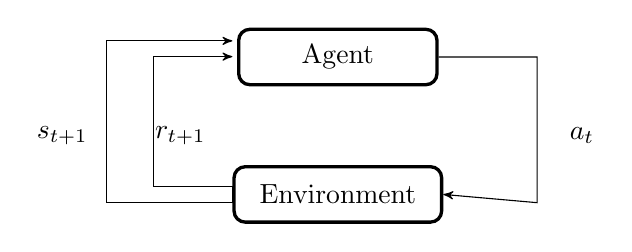
\begin{tikzpicture}[node distance=1cm, auto,]
      \node[punkt] (agent) {Agent};
      \node[punkt, inner sep=5pt,below=1cm of agent] (env) {Environment};
      \path[draw,->] 
        (env.west) -- ++(0cm,.1cm)  -- ++(-1cm,0cm) -- ++(0,1.65cm)  -- ++(1cm,0cm);
      \path[draw,->] 
        (env.west) -- ++(0cm,-.1cm) -- ++(-1.6cm,0cm) -- ++(0,2.05cm) -- ++(1.6cm,0cm);

      \path[draw,->] 
        (agent.east) -- ++(1.25cm,0cm) -- ++(0,-1.85cm) -- (env.east);


      \draw (3.1,-1) node[] {\( a_{t} \)};
      \draw (-2,-1) node[] {\( r_{t+1} \)};
      \draw (-3.5,-1) node[] {\( s_{t+1} \)};
  \end{tikzpicture}
  \caption[Agent enviroment interaction dynamic: ]%
  {\label{img:a-e_dynamic}Agent enviroment interaction dynamic: \small \textit{this is the basic dynamic of the interaction between the agent and the enviroment in a MDP, at time t the agent provides an action a and the enviroment respond with a state s and rewad r that are used from the agent to decide the action at t+1 and so on.}}
\end{figure}


\paragraph{Objective and Rewads:} The main objective of RL is to maximize the total number of rewars it receive. This reward \( r_t \) is passed from the environment to the agent at every timestep as a consequence of his actions. In the case of the Gather and Trade the reward is \( r_{i,t} = u_i(x_{i,t},l_{i,t})  - u_i(x_{i,t-1},l_{i,t-1}) \). 

Since the agents want to maximize the total upcoming reward we can write this value simply as the sum of all the future rewards.

\begin{equation*}
U_t \doteq r_{t+1} + r_{t+2} + ... + r_{H},
\end{equation*}

Where \( H \) is the total length of the episode, and at the time step \( t = H \) the episode ends. This state is called the terminal state and is a particular state because regardless of the final condition of the agent it reset the environment to the initial condition and restart completely the episode.
Another specification for the total reward can implement the concept of discounting, which is more appropriate in the case of economical simulations, thus within the experiments the agent has to maximize his future discounted utility:

\begin{equation}
U_t \doteq r_{t+1} + \gamma r_{t+2} + \gamma^2 r_{t+3} +... + \gamma^{H-t-1}r_{H},
\end{equation}

the discount rate \( \gamma \in [0,1] \) determines the value that the agent assigns to the future reward, a reward received at \( k \) timesteps in the future is only valued \(\gamma^{k-1} \) times what it would be valued today. When the value of \( \gamma \) approaches 0 the agent is more "myopic" and puts most of his interest in immediate rewards, while if it approaches 1 the interest is more projected in the future due to the stronger impact of future rewards.

\paragraph{Value functions: } One of the most important elements of RL is the value function. The estimation of this function is one of the crucial points of RL, in fact it tries to quantify the expected return of the rewards it expects to receive. Furthermore, the expected reward depends on the action that the agent decides to take, thus the value function are defined in terms of policies, which are acting behaviors.

If the agent is following policy \( \pi \) at time \( t \), then \( \pi(a|s) \) is the probability that the agent takes the action \( a_t = a \) given the state \( s_t = s \). The aim of RL is to change the policy based on experience across episodes to find an optimal behavior.

We can write a value funciton for a state \( s \) under the policy \( \pi \). This function is the expected return when the inital state is \( s \) and the policy followed is \( \pi \).

\begin{equation}
v_\pi(s) \doteq \mathbb{E} _\pi \left[ U_t | s_t = s \right] \, =\,  \mathbb{E} _\pi \left[\left.\sum_{k = 0}^{H}\gamma^k r_{t+k+1}  \right| s_t = s \right], \quad \text{for all}\, s \in \mathcal{S} 
\label{eq:statevalue_function}
\end{equation}

\(  v_\pi(s)\) is called the state-value function for policy \( \pi \). Following from this equation, it is possible to define the value of taking an action \( a \) in the state \( s \) following the policy \( \pi \):

\begin{equation}
    q_\pi(s,a) \doteq \mathbb{E} _\pi \left[ U_t | s_t = s, a_t = a \right] \, =\,  \mathbb{E} _\pi \left[\left.\sum_{k = 0}^{H}\gamma^k r_{t+k+1}  \right| s_t = s, a_t = a \right],
    \label{eq:actionvalue_function}
\end{equation}
    
and \( q_\pi(s,a) \) is called the action-value function for policy \( \pi \). The important concept here is that the value functions in \ref{eq:statevalue_function} and \ref{eq:actionvalue_function} can be estimated from experience. 

There are multiple strategies to determine an optimal behavior starting from the evaluation of these functions, we can divide these ways in two main groups, tabular solution methods and approximate solution methods\cite{sutton2018reinforcement}. For the former we have Montecarlo methods, Dynamic programming, Temporal-difference learing, n-step bootsrap and others. While for the latter we have On/Off-policy methods with approximation and policy gradient methods. 

For the purpose of this thesis we are going to foucs only on policy gradient methods and a particular set of optimization policy called proximal policy optimization.

\section{Approximate solution Methods}

The approximate solution methods are sets of strategies thought for those problems, such as ours, where the set of possible states is enormous. It is very likely that every state encountered in a simulation will never have been encountered before. Thus, to make meaningful decisions there is the need to be able to generalize from previous state that are, to some extent, similar. This is accomplished by borrowing the exising generalization theory, usually by using the process of function aproximation. However, we are going to use policy gradient methods that do not necessarily need to estimate a value function through function aproximation. 



\subsection{Policy gradient Methods}  


Policy gradient methods are a set of parameterized policies that can select actions without the use of a value function. The method consists in calculating the estimator of the policy gradient and feeding it into a stochastic gradient ascent algorithm. We denote with \( \pi_\theta(a|s) \) the stochastic policy such that 
\begin{equation}
  \pi_\theta(a|s) = \pi(a| s, \mathbf{\theta}) = Pr \left\{ a_t = a | s_t = s \, , \,   \mathbf{\theta}_t =  \mathbf{\theta}\right\}
\end{equation}
for the probability of choosing action \( a \) at time \(  t \) given the state \( s_t \) and the parameters \(  \mathbf{\theta} \). The aim of the policy gradient methods is to maximize a perfomance measure \( J_t( \mathbf{\theta}) \). This is done by updating the parameters \(  \mathbf{\theta} \) with a gradient of the performance itself:

\begin{equation}
  \mathbf{\theta}_{t+1} =  \mathbf{\theta}_t + \alpha\widehat{\nabla J ( \mathbf{\theta}_t)}
\end{equation}



\subsection{Proximal Policy Optimization Algorithms}

Proximal policy optimization algorithms (PPOs) are a family of policy gradient methods for reinforcement learning, which alternate between sampling data through interaction with the environment, and optimizing a "surrogate" objective function using stochastic gradient ascent. 

PPO utilizes as a performance measure the advantage \( A(s,a) = q(s,a) - v(s) \), which represents how good an action is compared to the average action in a specific state.

It also relies on the ratio of the policy that we want to refine to the older policy:

\begin{equation}
r_t(\theta)= \frac{\pi_\theta(a_t|s_t)}{\pi_{\theta old}(a_t|s_t)}
\end{equation}

The surrogate objective function that we optimize with PPO is 

\begin{equation}
\mathcal{L}^{CLIP} (\theta) = \hat E_t \left[ min(r_t(\theta)\hat A_t \,, \, clip(r_t(\theta) \,,\, 1-\epsilon\,,\, 1+ \epsilon)\hat A_t)\right]
\end{equation}

The maximization of this surrogate funcition takes the advantages of trust region policy optimization (TRPO) \cite{schulman2015high}, adjusting the parameters in the dierction of the ratio \( r_t(\theta) \), and maintaining this change bounded in a "clipped" region to avoid drastic refinements of the policy. This is shown well in the Figure \ref{img:l_clip}


\begin{figure}[h!]
  \centering
  \linespread{.9} 
  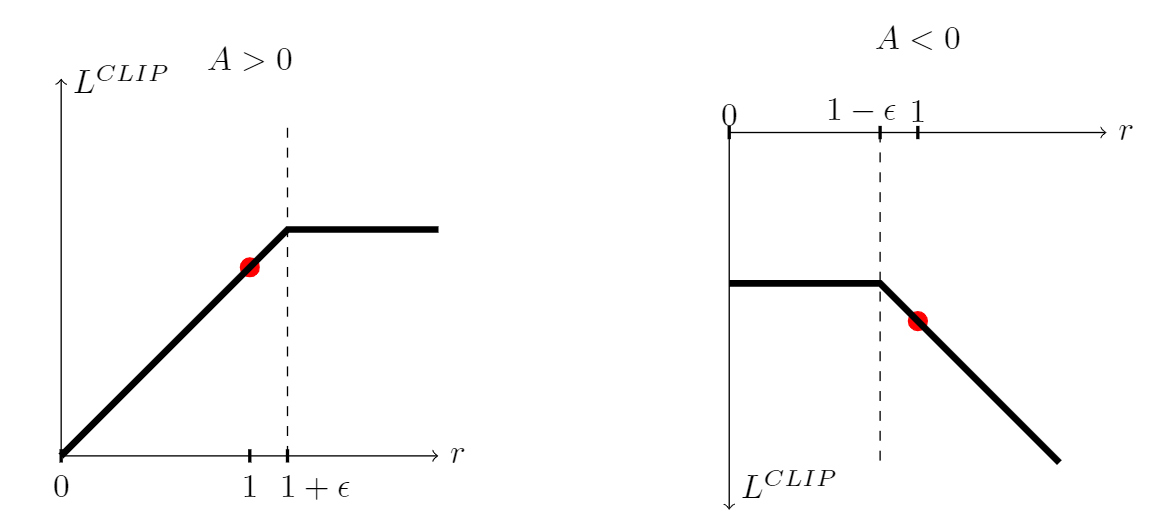
\includegraphics[width=0.75\textwidth]{Resources/imgs/L_clip.PNG}
  \caption[One step \( L^{CLIP} \) as a function of \( r_t(\theta) \):  ]%
  {\label{img:l_clip}One step \( L^{CLIP} \) as a function of \( r_t(\theta) \): \small \textit{this is the function \( L^{CLIP} \) as a function of the probability ratio \( r_t(\theta) \) when the advantage A is positive or negative. The red dot is the starting point of the optimization. (Figure from \cite{schulman2017proximal})}}
\end{figure}


The surrogate function can be further augmented by adding an entropy bonus to ensure sufficient exploration. By adding these terms, we obtain the following objective function:

\begin{equation}
L_t^{CLIP+VF+S}(\theta) = \hat E_t \left[ L_t^{CLIP}(\theta) - c_1 L_t^{VF}(\theta)  + c_2 S[\pi_\theta](s_t)\right]
\end{equation}

where \( S \) in an entropy bonus, \(  L_t^{VF} \) is a squared-error loss and \(c_1, c_2 \) are coefficients.

The pseudocode below better explains all the procedure done by the PPO in refining the parameters.

\begin{algorithm}
  \caption{PPO with clipped objective}\label{alg:ppo_clip}
  \begin{algorithmic}
    \State Input: inital policy \( \theta_0 \), clipping threshold \( \epsilon \)
    \For{\( k = 0,1,2... \)}
      \State Collect a set of trajectories $\mathcal{D}_k$ on policy \( \pi_k = \pi(\theta_k) \)
      \State Estimate the adventages \( \hat A_t^{\pi_k} \), using any advantage est. alg. 
      
      \Comment{we will use GAE\cite{schulman2015high}}
      \State Compute policy update
      \begin{equation*}
        \mathbf{\theta}_{k+1} = arg \max_\theta \mathcal{L}^{CLIP}_{\theta_k}(\theta)
      \end{equation*}
      \State by taking K steps of minibatch SGD (via Adam \cite{kingma2014adam}), where
      \begin{equation*}
        \mathcal{L}^{CLIP}_{\theta_k}(\theta) =  E_t \left[ \sum_{t=0}^T\left[  min(r_t(\theta)\hat A^{\pi_k}_t \,, \, clip(r_t(\theta) \,,\, 1-\epsilon\,,\, 1+ \epsilon)\hat A_t^{\pi_k})\right]\right]
      \end{equation*}
    \EndFor
  \end{algorithmic}
\end{algorithm}



\begin{comment}

One of the most often used gradient estimator uses the following formula:

\begin{equation}
\hat g = \hat E_t \left[ \nabla_\theta log \pi_\theta ( a_t | s_t) \hat J_t  \right]
\end{equation}

Here the expected value is taken over a minibatch in an algorithm that alternates sampling and optimization.

  \bigskip


\begin{algorithm}
  \caption{basic PPO structure}\label{alg:cap}
  \begin{algorithmic}
      \For{iteration = 1,2 ...}
      \For{actor = 1,2,..., N}
        \State Run policy \( \pi_{\theta_{old}} \) in enviroment for \( T \) time-steps
        \State Compute advantage estimate \( \hat A_1 , ... , \hat A_T \)
      \EndFor
      \State Opt. surrogate \( L \) wrt \( \theta \), with K epochs and minibatch size \( M \leq NT \)
      \State $\theta_{old} \gets \theta$
    \EndFor
  \end{algorithmic}
\end{algorithm}

\end{comment}




 
%------------------------------------------------------------------------------------




%------------------------------------------------------------------------------------
% CHAPTER 3
%------------------------------------------------------------------------------------
%\chapter{Optimal taxation}
%\textcolor{red}{ future work}

\begin{itemize}
    \item Simualting the concept of tax evasion
    \item simulating coexisting tax and migration of high skilled agents
    \item simualtion with RL policymaker
    \item 
\end{itemize}
%------------------------------------------------------------------------------------



%------------------------------------------------------------------------------------
% CHAPTER 4 
%------------------------------------------------------------------------------------
\chapter{Experiments}
In this chapter I will present the two phases learning process utilized by the fully connected neural network (FCNet) to maximize the agents utility. Afterwards there will be a brief description of the 5 environments I am going to study (one per taxation analyzed) and my conjecture on how the agents will respond to these taxation.


\section{Experiment Setup}

After understanding the Foundation framework and the process used by RL to optimize a policy we can focus on the model used. In the paper used as a reference the authors used a combination of a convolutional neural network and a LSTM \cite{zheng2020ai}. This could grant them good spatial information from the CNN and a memory buffer from the LSTM. These feature are sensate because there is the need of process a map and because the agents share the same network.

In the experiments, however, it was used a fully connected neural network that do not share the same feature as the one above. The complete stucture of the model is shown in Table \ref{tab:Fcnet}. 


\begin{table}[h!]
    \begin{tabular}{llll}
	Model: "FCNet"            &                    &          &                            \\ \hline
	Layer (type)              & Output Shape       & Param \# & Connected to               \\ \hline
	observations (InputLayer) & {[}(None, 1260){]} & 0        &                            \\ \hline
	encoder (Encoder)         & (None, 256)        & 389632   & observations{[}0{]}{[}0{]} \\ \hline
	fc\_out (Dense)           & (None, 50)         & 12850    & encoder{[}0{]}{[}0{]}      \\ \hline
	value\_out (Dense)        & (None, 1)          & 257      & encoder{[}0{]}{[}0{]}      \\ \hline
	Total params: 402,739     &                    &          &                            \\
	Trainable params: 402,739 &                    &          &                            \\
	Non-trainable params: 0   &                    &          &                            \\ \hline
    \end{tabular}
    \caption{\label{tab:Fcnet} Fully connected neural network utilized.}
\end{table}


This setup might encur in a loss of efficiency for plenty of reasons. First of all, as said before, the feature of the LSTM/CNN are missing. Then due to lack of resources it was not possible to do a proper hyper parameter tuning, probably leading to inefficiencies. However, as we will see, the FCNet can provide us with meaningful results, in particular the agents will show emerging behaviors and specialization. These are feature that were also finded in the paper by Zhang and Trott, the difference is present in the efficiency of the agents that is lower for the model used here.

There are many parameters that have to be set at this stage (for a semi-complete list check the appendix \textcolor{red}{appendice}). A first part of these values are related to the training, while a second part to the environment. I would like to stress some of the latter parameters, to better undersand the simulation.

First the skill levels, these are set to be different for each agent, the skill is the amount of coins received when building an house. The set of 4 skills is fixed and these are taken from a pareto distribution. Namely the values are (11.3; 13.3; 16.5; 22.2). These value are always assinged to the same starting location in the map, thus the agent starting in the bottom right will always have the highest skill and so on. Other important parameters are the episode lenght \( H \) which is set to 1000 time steps, the resource respawn probability which is set to 1\% per timestep and the inital coin endowment that is set to 0.

Once defined the environment is defined it is possible to start the training, this will happen in two phases. The first phase to introduce labour, and the second to introduce the taxation.

\section{Phase 1 training}

The first training phase is necessary in order to get the FCNet \ref{tab:Fcnet} accustomed to the world dynamics and avoid falling into unoptimal behavior once disincentives factors are introduced. These two factors, as already discussed, are labour costs and taxation. In this first phase the interest is in getting the agent accustomed to the labour costs, while the taxes are completely removed and will be investigated in the second phase of training. 


\begin{figure}[h!]
    \centering
    \linespread{.9} 
    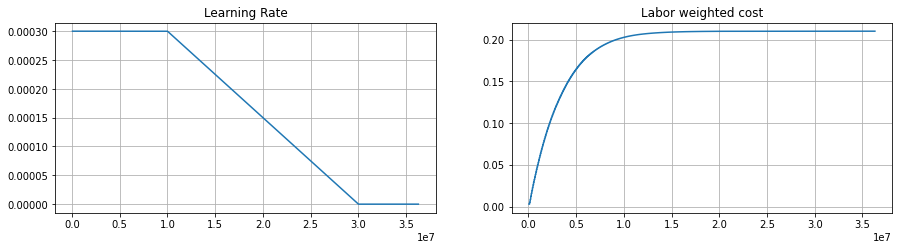
\includegraphics[width=0.95\textwidth]{Resources/imgs/LR_phase1.png}
    \caption[Learning rate and Labor weighed cost for Phase 1 training: ]%
    {\label{img:lr_phase0}Learning rate and Labor weighed cost for Phase 1 training: \small \textit{this was the schedule for respectively the learning rate and the labor cost in the phase 1 of the training, here the learning rate goes to 0 because we don't seek convergence now.}}
\end{figure}

The training agenda is built to run for a total of 30M time-steps, as we can see from Figure \ref{img:lr_phase0} the learning rate is set to be at 1e-4 for 10M steps then it linearly reduces to 0 in 20M time-steps. While the labour weight increases following the function:

\begin{equation}
    \vartheta_k = 1- exp\left(- \frac{\textit{episode completitions}}{\textit{energy warm-up constant (k)}}\right)
\end{equation}

where the warm-up constant is set to 10000. This setup gives the FCNet time to learn how to respond properly to the dis-utility generated by the labor. 



\begin{figure}[h!]
    \centering
    \linespread{.9} 
    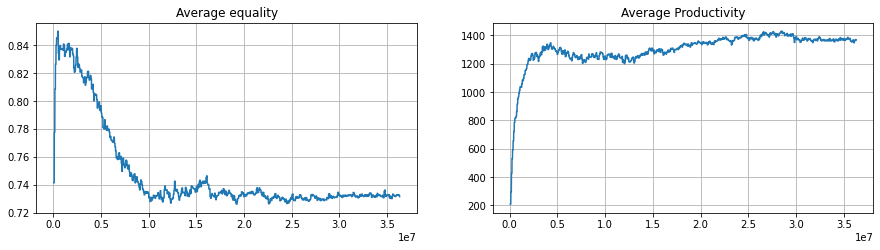
\includegraphics[width=0.95\textwidth]{Resources/imgs/FCNET_prod_phase1.png}
    \caption[Equality and Productivity during Phase 1:  ]%
    {\label{img:prod_phase0}Equality and Productivity during Phase 1: \small \textit{here we have the evolution of equality between agents and total production in the training of phase 1}}
\end{figure}


In Figure \ref{img:prod_phase0} we can see two of the most important variables that we are considering. On the left we have the average equality, this value is calculated by the following formula:

\begin{equation}
    equality(\mathbf{x^c_{t}}) = 1 - \frac{N}{N-1} \frac{\sum^N_{i=1}\sum^N_{j=1}| x^c_{i,t} - x^c_{j,t}|}{2N\sum^N_{i=1}x^c_{i,t}}
\end{equation}

with \( 0 < equality(\mathbf{x^c_{t}}) < 1 \), this function returns 1 if the endowments are equally split between the N (4) agents, and 0 if only one agent owns all of the coin in the economy. What we see is that after 36M time-steps the equality settled around 0.73, this is justified by the difference in coin endowment between the agent with the highest skill (Agent 0 in Figure \ref{img:p0_brakedown}) and the other agents. And we see that the average productivity of he economy settles around 1400. 


\begin{figure}[h!]
    \centering
    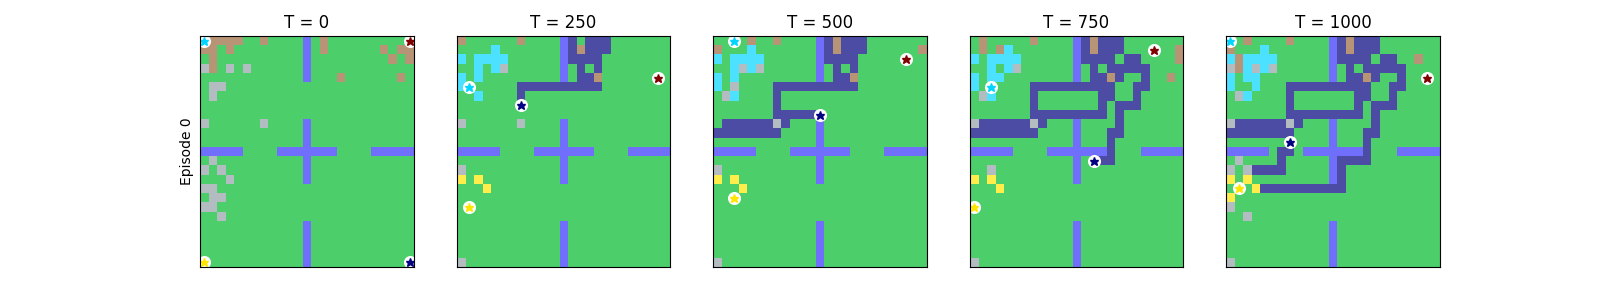
\includegraphics[width=0.95\textwidth]{Resources/imgs/Figure_1.png}
    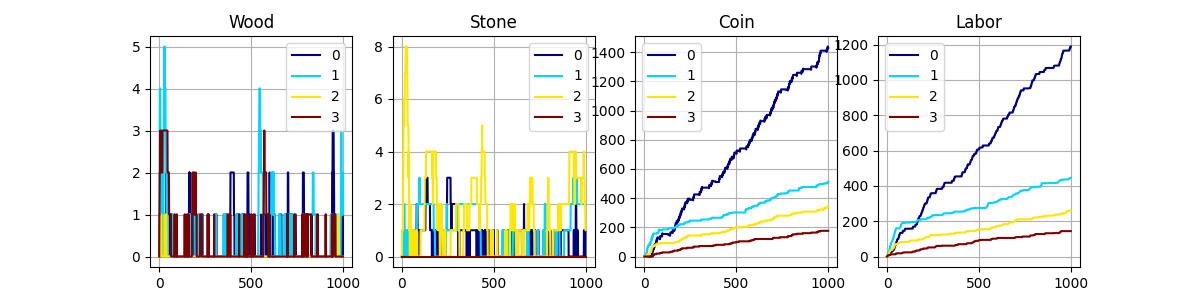
\includegraphics[width=0.80\textwidth]{Resources/imgs/Figure_2.png}
    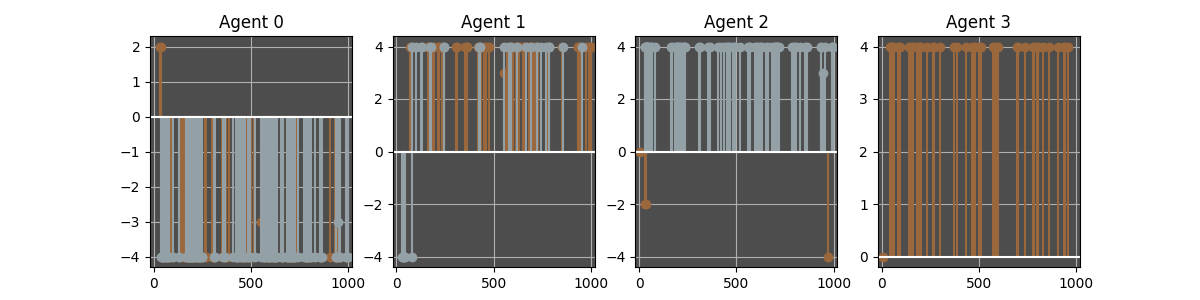
\includegraphics[width=0.80\textwidth]{Resources/imgs/Figure_3.png}
    \caption[Phase 1 full brake down: ]%
    {\label{img:p0_brakedown}Phase 1 full brake down: \small \textit{this is a more complete overview of one random simulation crated using the weights at the end of phase 1 training}}
\end{figure}


The results obtained so far are not important for the final analysis since there were no criterion used to stop the training other than a time constraint. This means that the FCNet might have not reached convergence and an optimal policy. However we can keep these results in mind as a benchmark for the phase 2 trainig as we will use the parameters obtained to carry on the training.


\section{Phase 2 Trainig}

    
In the second phase of the training the learning rate schedule is changed to be 3e-4 for the first 35M time-steps and then will linearly decrease to 1e-6 in a span of 15M time-steps. This will grant a faster learning rate in the inital part of the trainig when the FCNet will suffer a huge decrease in efficiency due to the introduction of the taxation. 

The starting point for this second phase are the weights obtained from phase 1, and the training will be formed of five different simulations diverging from this inital state. These simulation are: US taxation, Italian Taxation, free market, Communism and Flat Tax.

\subsection{Free Trade}

Free trade is the first and simplest kind of simulation that we can carry on starting from the result in phase 1. This training consist in keep training the FCNet without imposing any kind of taxation. 

It is reasonable to belive that the result of this first training should produce a more productive economy since the agent's utility function is positive in marginal coin endowment. However the equality between agents might suffer from a higher production.

\subsection{US taxation}

The second kind of taxation that will is used is the US taxation. This is based on the 2018 Federal brachets and percentages. In particular we can see from Table \ref{tab:us_tax} the detailed stucture. 

\begin{table}[h!]
\begin{adjustbox}{max width=\textwidth}
    \begin{tabular}{llllllll}
        \hline
    Bracket in \$   & 0-9700 & 9700-39475 & 39475-84200 & 84200-160725 & 160725-204100 & 204100-510300 & 510300+ \\
    Bracket in Coin & 0-9.7  & 9.7-39.5   & 39.5-84.2   & 84.2-160.7   & 160.7-204.1   & 204.1-510.3   & 510.3+  \\
    Tax*            & 10\%   & 12\%       & 22\%        & 24\%         & 32\%          & 35\%          & 37\%\\
    \hline
    \end{tabular}
\end{adjustbox}
    \caption[2018 US federal tax system:]%
    {\label{tab:us_tax}2018 US federal tax system: \small \textit{this is the proportional system that was in place in the US in 2018, notice that the tax is marginal (i.e. if you are in the second bracket you will pay 970\$ + 12\% of the amount above 9700\$) }}
\end{table}

With the introduction of these lump sum tax plus redistribution is easy to conclude that there might me an increase in equality, however this migh produce a negative effect on total production since the high-skilled agent are disincentivised to produce.

\subsection{Italian Taxation}

As of the US's the Italian is a marginal system with brackets, however in this case the fiscal pressure is higer and the brachets smaller. As a reference it was used the 2020 INPS brachets and percentages (Table \ref{tab:ita_tax}). However, the brackets were calculated as if in dollars, so all the values were multiplied by 1.1575, the exchange rate at October 1st 2021.


\begin{table}[h!]
    \begin{adjustbox}{max width=\textwidth}
        \begin{tabular}{llllll}
            \hline
        Bracket in \EURcr   & 0-15000 & 15000-28000 & 28000-55000 & 55000-75000 & 75000+ \\
        Bracket in Coin & 0-17  & 17-32  & 32-63  & 63-86   &  86+   \\
        Tax*            & 23\%   & 27\%       & 38\%        & 41\%         & 43\%       \\
        \hline
        \end{tabular}
    \end{adjustbox}
        \caption[2018 US federal tax system:]%
        {\label{tab:ita_tax}2020 INPS tax system: \small \textit{this is the proportional system that was in place in the Italy in 2020, notice that the tax is marginal (i.e. if you are in the second bracket you will pay 3450\EURcr + 27\% of the amount above 15000\EURcr) }}
    \end{table}



In this case there is an even higher pressure, wich might push toward higher equality and lower total production.


\subsection{Communism}

Communism is the opposite to Free market, in this simulation the fiscal pressure is 1, meaning that every 100 timestep all the agents are taxed for the entire amount of coins they own and then redistibuted. This system will probably deliver the loewst production and the highest equality.

\subsection{Flat tax}



\section{Training Results}


\begin{figure}[h!]
    \centering
    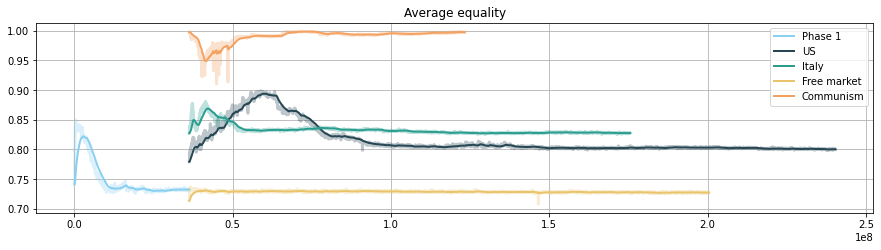
\includegraphics[width=0.95\textwidth]{Resources/imgs/equality_training.png}
    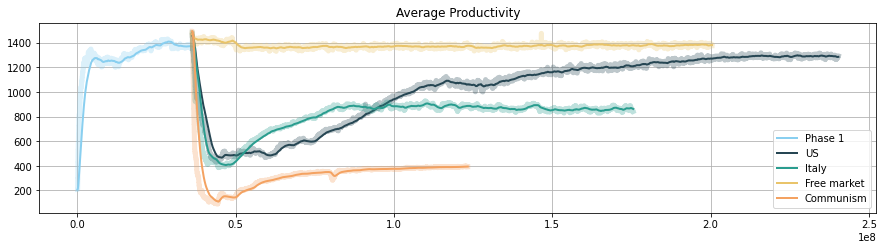
\includegraphics[width=0.95\textwidth]{Resources/imgs/productivity_training.png}
    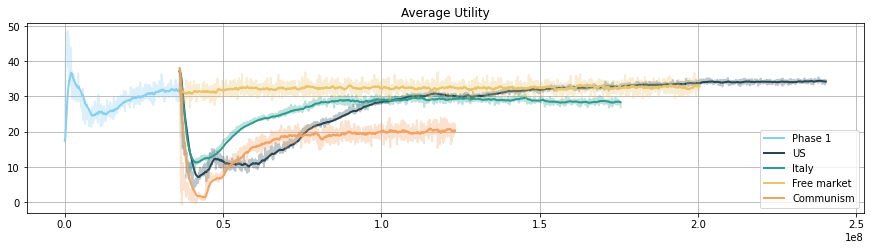
\includegraphics[width=0.95\textwidth]{Resources/imgs/utility_training.png}
    \caption[Phase 1 full brake down: ]%
    {\label{img:p1_brakedown}Phase 2 full brake down: \small \textit{this is a more complete overview of one random simulation crated using the weights at the end of phase 1 training}}
\end{figure}

%------------------------------------------------------------------------------------

%------------------------------------------------------------------------------------
% CHAPTER 5
%------------------------------------------------------------------------------------
\addcontentsline{toc}{chapter}{Conclusions}
\chapter*{Conclusions}

We have seen how reinforcement learning could be used to produce economical simulations. In detail, we saw RL applied to the gather-and-trade setup created by Alex Trott and Stephan Zheng. Here, we noticed how it is possible to maximize agents utility through proximal policy optimization, a kind of gradient descent optimization. And we saw how this gave birth to agents specialization, a feature that is hard to capture analytically. Afterwards we saw four different taxation system (and redistribution) applied to a common starting point and commented on the difference on productivity and equality. We found out, reasonably, that there is a negative impact of taxation on production and a positive impact on equality. This impact cannot be properly quantified as partial effect for a multitude of reasons. However it was possible to compare the results in performance terms. 




\subsection*{Future work}

This simulations can be a nice starting point for a multitude of future works. At first is possible to study the application of RL in simpler setup that can completely modeled in an analytical way and check if RL converges to the analytical solutions. Afterward, starting from this model, is possible to explore plenty scenarios. A couple that could be interesting in my opinion are the brain drain and tax evasion. For the former we could simulate two countries that coexist and we could give the agents the choice to move from country A to country B. Then we could study how the high and low skilled agents decide to move across the countries. For the latter is possible to add the choice to reveal the real income and a small possibility to being caught. Here the interest would be in if or how the agents decide to evade given different tax systems. 

These are just two examples, but the freedom of design is technically endless. Of course such research would need better machines, thus computational power, than the one's used for this thesis.
%------------------------------------------------------------------------------------







\renewcommand{\chaptermark}[1]{\markright{\thechapter \ #1}{}}
\lhead[\fancyplain{}{\bfseries\thepage}]{\fancyplain{}{\bfseries\rightmark}}
\appendix   
%\addcontentsline{toc}{chapter}{Appendix}
\chapter{Tables}  



\begin{table}[]
    \centering
    \begin{tabular}{lll}
    \hline
    Parameter                    &  & Value \\ \hline
    Episode Lenght               & \( H \) & 1000  \\
    World height                 &  & 25    \\
    World width                  &  & 25    \\
    Resources respawn prob.      &  & 0.01  \\
    Inital Coin endowment        &  & 0     \\
    Iso-elastic utility exponent &  & 0.23  \\
    Move labor                   &  & 0.21  \\
    Gather labor                 &  & 0.21  \\
    Trade labor                  &  & 0.05  \\
    Build labor                  &  & 2.1   \\
    Base build payout            &  & 10    \\
    Max skill multiplier         &  & 3     \\
    Max bid/ask price            &  & 10    \\
    Max bid/ask order duration   &  & 50    \\
    Max simultaneous open orders &  & 5     \\
    Tax period duration          &  & 100   \\
    Min bracket rate             &  & 0\%   \\
    Max bracket rate             &  & 100\% \\ \hline
    \end{tabular}
    \caption{\label{tab:hyperparameter_env}Your caption.}
\end{table}


\begin{table}[]
    \centering
    \begin{tabular}{lll}
    \hline
    Variable Name                                 & Dimension   & Bounds                      \\ \hline
    world Map                                     & (7, 11, 11) & \{0;1\}                     \\ 
    world-idx\_map                                & (2, 11, 11) & \{0,1,...,5\}               \\ 
    world-loc-row                                 & (1,)        & {[}0,1{]}                   \\ 
    world-loc-col                                 & (1,)        & {[}0,1{]}                   \\ 
    world-inventory-Coin                          & (1,)        & {[}0,inf)                   \\ 
    world-inventory-Stone                         & (1,)        &                             \\ 
    world-inventory-Wood                          & (1,)        &                             \\ 
    time                                          & (1, 1)      &                             \\ 
    Build-build\_payment                          & (1,)        &                             \\ 
    Build-build\_skill                            & (1,)        &                             \\ 
    ContinuousDoubleAuction-market\_rate-Stone    & (1,)        &                             \\ 
    ContinuousDoubleAuction-price\_history-Stone  & (11,)       &                             \\ 
    ContinuousDoubleAuction-available\_asks-Stone & (11,)       &                             \\ 
    ContinuousDoubleAuction-available\_bids-Stone & (11,)       &                             \\ 
    ContinuousDoubleAuction-my\_asks-Stone        & (11,)       &                             \\ 
    ContinuousDoubleAuction-my\_bids-Stone        & (11,)       &                             \\ 
    ContinuousDoubleAuction-market\_rate-Wood     & (1,)        &                             \\ 
    ContinuousDoubleAuction-price\_history-Wood   & (11,)       &                             \\ 
    ContinuousDoubleAuction-available\_asks-Wood  & (11,)       &                             \\ 
    ContinuousDoubleAuction-available\_bids-Wood  & (11,)       &                             \\ 
    ContinuousDoubleAuction-my\_asks-Wood         & (11,)       &                             \\ 
    ContinuousDoubleAuction-my\_bids-Wood         & (11,)       &                             \\ 
    Gather-bonus\_gather\_prob                    & (1,)        &                             \\ 
    action\_mask                                  & (50,)       &                             \\ \hline
    \end{tabular}
    \caption{\label{tab:full_obs} Full observation space.}
\end{table}
\rhead[\fancyplain{}{\bfseries \thechapter \:Tables}]
{\fancyplain{}{\bfseries\thepage}}


\nocite{ai-economist}
\nocite{aie_git}
\nocite{akira_git}
\nocite{akira_medium}
\nocite{my_git}

\printbibliography[type=article]
\printbibliography[type=online, heading=subbibliography, title=Sitography]
\printbibliography[type=online2, heading=subbibliography, title=Source Code]
\end{document}
